\subsection{Introduction}

In the previous sections, all of the preliminary components for
state estimation were discussed:
the Bayes filter as a foundation;
the motion and the measurement models based on the
sensors and the kinematics of the actual robot;
and the representation of the environment as an OGM.

The main goal of this section is to introduce the Exact Flow Daum Huang filter. However, to properly understand the motivation behind
the creation of the filter along with its strengths and weaknesses, first the
examination of the Kalman filters and the particle filters are necessary.

Besides that Kalman filters are essential to understand state estimation,
the extended Kalman Filter (EKF) is directly required for the implemented Daum--Huang filter variant. For this special localization task with
an implicit measurement equation, the implicit extension of the EKF is provided, based on the literature.

As Daum--Huang filters are mainly developed to specifically overcome
an important deficiency of particle filters, their detailing is
also required. This is done through the examination of the bootstrap particle filter algorithm.

Finally, the Daum--Huang filters are discussed in general,
followed by the Exact Flow Daum--Huang filter (EDH). Similarly to the EKF,
an implicit extension is also required here to suit the
specific localization task. Such method is  yet not to be found in the literature, therefore lies within the contributions
of this report.
\subsection{The Kalman Filters}
\subsubsection{Kalman Filter}
The Kalman filter (KF) assumes that ``everything'' \emph{is} linear and Gaussian,
and under these assumptions it can be proved that ``everything'' \emph{stays} linear and Gaussian during the Bayes filter updates.
A Gaussian distribution can be fully characterized by its first two moments,
therefore the Kalman filter offers a recursion to calculate the mean $\boldsymbol{\mu}_t$ and the covariance $\mathbf{\Sigma}_t$ of the belief $bel(\mathbf{x}_t)$.
In this context only the discrete-time KF is going to be discussed.

Consider the discrete-time (linear) state space model of a controlled system:
\begin{align}
    \mathbf{x}_t & = \mathbf{A}_t\mathbf{x}_{t-1} + \mathbf{B}_t\mathbf{u}_t + \mathbf{B}_t\mathbf{v}_t, \\
    \mathbf{z}_t & = \mathbf{C}_t\mathbf{x}_t + \mathbf{w}_t, \label{eq:lin-meas-model}
\end{align}
% ! TODO v és w kicserél
where $\mathbf{A}_t$ is the state transition matrix, $\mathbf{B}_t$ is the input gain, and $\mathbf{C}_t$ is the measurement matrix. To incorporate uncertainties and inaccuracies into the system,
the control noise $\mathbf{v}_t$ and the measurement noise $\mathbf{w}_t$ is introduced.
Both are Gaussian random variables:
$\mathbf{v}_t \sim \mathcal{N}(\mathbf{0},\mathbf{Q})$, $\mathbf{w}_t \sim \mathcal{N}(\mathbf{0},\mathbf{R})$,
with $\mathbf{Q}$ as control noise covariance, and $\mathbf{R}$ as measurement noise covariance.

Using the linear nature of the model, and assuming, that the probability distributions in the Bayes filter are Gaussian distributions, the motion model has the following form:
\begin{equation}\label{key}
    p(\mathbf{x}_t|\mathbf{x}_{t-1}, \mathbf{u}_t) = \mathrm{det}(2\pi\tilde{\mathbf{Q}}_t)
    ^{-\frac{1}{2}}\mathrm{exp}\{-\frac{1}{2}(\mathbf{x}_t-\mathbf{A}_t\mathbf{x}_{t-1}-
    \mathbf{B}_t\mathbf{u}_t)^\top\tilde{\mathbf{Q}}_t^{-1}(\mathbf{x}_t-\mathbf{A}_t\mathbf{x}_{t-1}-\mathbf{B}_t\mathbf{u}_t)\},
\end{equation}
where $\tilde{\mathbf{Q}}_t = \mathbf{B}_t\mathbf{Q}_t\mathbf{B}_t^{\top}$.
The measurement model can be calculated similarly.

The derivation of the Kalman filter algorithm is not trivial, and does not fall within the scope of this document. The algorithm can be seen in Algorithm \ref{alg:kf}., where $\mathbf{I}$ denotes the identity matrix, $\mathbf{z}'_t$ is the actual measurement.

\begin{algorithm}
    \caption{Kalman filter($\boldsymbol{\mu}_{t-1},\mathbf{\Sigma}_{t-1},\mathbf{u}'_t,\mathbf{z}'_t$)}\label{alg:kf}
    \begin{algorithmic}[1]
        \BState \emph{prediction}:
        \State\indent$\overline{\boldsymbol{\mu}}_t = \mathbf{A}_t{\boldsymbol{\mu}}_{t-1} + \mathbf{B}_t\mathbf{u}'_t$
        \State\indent $\overline{\mathbf{\Sigma}}_t = \mathbf{A}_t\mathbf{\Sigma}_{t-1}\mathbf{A}^\top_t + \tilde{\mathbf{Q}}_t$
        \BState \emph{update/correction}:
        \State\indent $\mathbf{K}_t = \overline{\mathbf{\Sigma}}_t\mathbf{C}_t^\top\left(\mathbf{C}_t\overline{\mathbf{\Sigma}}_t\mathbf{C}_t^\top+\mathbf{R}_t\right)^{-1}$
        \State\indent $\boldsymbol{\mu}_t = \overline{\boldsymbol{\mu}}_t + \mathbf{K}_t\left(\mathbf{z}'_t-\mathbf{C}_t\overline{\boldsymbol{\mu}}_t\right)$
        \State\indent $\mathbf{\Sigma}_t = \left(\mathbf{I}-\mathbf{K}_t\mathbf{C}_t\right)\overline{\mathbf{\Sigma}}_t$
        \State\Return $\boldsymbol{\mu}_t,\mathbf{\Sigma}_t$
    \end{algorithmic}
\end{algorithm}
\subsubsection{Extended Kalman Filter}
However, assuming a linear state space model is a rather strong assumption. For a nonlinear model the general state space equations are:
\begin{align}
    \mathbf{x}_t & = \phi(\mathbf{x}_{t-1},\mathbf{u}_t,\mathbf{v}_t) \label{eq:explicit-mot-eq} \\
    \mathbf{z}_t & = \psi(\mathbf{x}_t,\mathbf{w}_t).  \label{eq:explicit-meas-eq}
\end{align}
The state propagation function $\phi$ can be locally linearized about $\mathbf{x}_{t-1} = \boldsymbol{\mu}_{t-1}, \mathbf{u}_t = \mathbf{u}'_t$ with respect to $\mathbf{x}_{t-1}$ and $\mathbf{u}_t$, resulting in $\nabla \phi _x(\boldsymbol{\mu}_{t-1},\mathbf{u}'_t)$ and $\nabla \phi_u(\boldsymbol{\mu}_{t-1},\mathbf{u}'_t)$.
The measurement function $\psi$ is linearized about the current predicted state $\overline{\boldsymbol{\mu}}_t$,
resulting in $\nabla \psi_x(\overline{\boldsymbol{\mu}}_t)$.
In Algorithm \ref{alg:ekf}., the arguments of these Jacobians are omitted.

As a summarization, the EKF algorithm (see in Algorithm \ref{alg:ekf}.) is the extension of the KF by handling nonlinear state equations through their Jacobians.

\begin{algorithm}
    \caption{Extended Kalman filter($\boldsymbol{\mu}_{t-1},\mathbf{\Sigma}_{t-1},\mathbf{u}'_t,\mathbf{z}'_t$)}\label{alg:ekf}
    \begin{algorithmic}[1]
        \BState \emph{prediction}:
        \State\indent$\overline{\boldsymbol{\mu}}_t = \phi(\boldsymbol{\mu}_{t-1},\mathbf{u}'_t,0)$
        \State\indent $\overline{\mathbf{\Sigma}}_t = \nabla \phi_x\mathbf{\Sigma}_{t-1}\nabla \phi_x^{\top} +
            \nabla \phi _u\mathbf{Q}_t \nabla \phi_u^{\top}$
        \BState \emph{update/correction}:
        \State\indent $\mathbf{K}_t = \overline{\mathbf{\Sigma}}_t\nabla \psi_x^\top\left(\nabla \psi_x\overline{\mathbf{\Sigma}}_t\nabla \psi_x^\top+\mathbf{R}_t\right)^{-1}$ \label{alg:line:kalman-gain}
        \State\indent $\boldsymbol{\mu}_t = \overline{\boldsymbol{\mu}}_t + \mathbf{K}_t\left(\mathbf{z}'_t-\psi(\overline{\boldsymbol{\mu}}_t,0)\right)$ \label{alg:line:state-update}
        \State\indent $\mathbf{\Sigma}_t = \left(\mathbf{I}-\mathbf{K}_t\nabla \psi_x\right)\overline{\mathbf{\Sigma}}_t$
        \State\Return $\boldsymbol{\mu}_t,\mathbf{\Sigma}_t$
    \end{algorithmic}
\end{algorithm}

\subsubsection{EKF for Implicit Measurement Equation}

The standard KF and EKF assume an explicit measurement equation in the form of \eqref{eq:explicit-meas-eq}.
However, as stated in Subsection \ref{subsec:dt-meas-model}, the measurement equation for the inspected
localization problem has an implicit form of \eqref{eq:impl-meas-eq}.
To suit this condition, Algorithm \ref{alg:ekf}. has to be modified, based on \cite{Steffen2013,Zhang2012}.
Line \ref{alg:line:kalman-gain}. is changed to
\begin{equation}
    \mathbf{K}_t = \overline{\mathbf{\Sigma}}_t\nabla \psi_x^\top\left(\nabla \psi_x\overline{\mathbf{\Sigma}}_t\nabla \psi_z^\top+
    \nabla \psi_z\mathbf{R}_t\nabla \psi^{\top}_z\right)^{-1},
\end{equation}
where $\nabla \psi_z$ is the Jacobian of $\psi$ with respect to $\mathbf{z}_t$, evaluated at
$\mathbf{x}_t = \overline{\boldsymbol{\mu}}_t, \mathbf{z}_t = \mathbf{z}'_t$.
Furthermore, because the expected output of the observation function is 0, Line \ref{alg:line:state-update}. has the modified form
\begin{equation}
    \boldsymbol{\mu}_t = \overline{\boldsymbol{\mu}}_t + \mathbf{K}_t\left(0-\psi(\overline{\boldsymbol{\mu}}_t,\mathbf{z}'_t)\right).
\end{equation}
\subsubsection{Advantages and Disadvantages of Kalman Filters}

Under linear and Gaussian assumptions the Kalman filter yields the optimal estimation (by calculated mean square error). However, these criteria are rarely satisfied, and the optimal estimation property does not hold any more. Another major problem comes from the nature of Gaussian distributions: they are unimodal, therefore the Kalman Filter cannot track multiple high-probability hypotheses.

EKF offers one type of solution to the nonlinearity: linearization by Taylor expansion. This however, introduces linearization error into the system. For highly nonlinear equations not only the first order approximation is the problem, but its center point as well. As were mentioned before, the state equation is linearized around the previous state; but now this state also an approximation. This overall effect can cause the algorithm to diverge, or to yield poor results. In addition, the initial conditions also have to be carefully chosen in order to obtain desired results.

Despite these, the EKF is still one of the most popular state estimation algorithm in robotics, and often used in Global Navigation Satellite Systems (GNSS) as well, thanks to its computational simplicity and easy  implementation. Other Kalman filter based realizations are including but not limited to the unscented Kalman filter (UKF), which uses a different type of linearization instead of the Taylor expansion based one, and the ensemble Kalman Filter (EnKF), which is suited for high dimensional estimation problems.

\subsection{The Particle Filters}
\subsubsection{Main concepts}

Particle filters (PF) are used to solve nonlinear filtering problems. Unlike EKF and other nonlinear extensions of the Kalman filter, this method uses a nonparametric representation of the estimated posterior. This nonparametric nature enables the estimation of various distributions, including multimodal and/or non-Gaussian.

The main concept in PF is to represent arbitrary probability distributions by cumulative probability mass of particles. When for example a Gaussian distribution is sampled multiple times, more samples come from regions with high probability density. This (trivial) effect can also be used in reverse: if samples are given, what is the probability distribution from which they were sampled? If the number of particles is sufficiently large (ideally infinity), they can offer a good approximation of the generating probability distribution.

The Bayesian filtering framework is implemented as follows. First, draw $N$ samples (called as particles) from a prior distribution. Then migrate each of these particles according to the motion model. Now the particle set will approximately describe the predicted belief \eqref{eq:predbel}. (In the KF this predicted belief was described by its mean and covariance, as it was assumed to be a Gaussian distribution. Now, it is described by particles, and the Gaussian nature is not required.)

The KF used the $\mathbf{K}_t$ Kalman gain as a weight to calculate the posterior from the predicted belief. Particle filters use \emph{importance sampling} for this task: each sample is given an importance weight which describes its relevance. If this relevance is high, it means that the specific particle is a good approximation of the true (sought) state. Choosing a proper weighting method is a difficult task. Generally, weights are calculated from a target and a proposal distribution. The target distribution is the posterior, the proposal distribution however, can be arbitrary (under some criteria). Now using the particles and their weights, the posterior distribution is approximated.

The next step of the filter is optional, although essential: resampling. Here, a new (same sized) particle set is constructed by drawing particles from the old set with replacement, according to their weights. This means that some  particles can be chosen multiple times (more likely high-weighted ones), thus certain particles can be eliminated. Finally, their weights are equalized. With the resulting particle set (either the new, redrawn one, or the old, weighted one), the algorithm is repeated in the new time step.

Generally, the most demanding task when designing PFs is the proper selection of the proposal density and the resampling frequency (i.e. when to resample). Choosing the right proposal distribution and the right time to resample is crucial in the performance of the PF. In the next subsection, the bootstrap particle filter method with adaptive resampling is introduced in detail.
\subsubsection{The Bootstrap Particle Filter}

Denote the particles and their set at time $t$  as:
\begin{equation}\label{key}
    \mathcal{X}_t = \{\mathbf{x}_t^{[1]},\mathbf{x}_t^{[2]}, \dots \mathbf{x}_t^{[N]}\}.
\end{equation}

The bootstrap particle filter uses the predicted belief as the proposal distribution, which results in the following weight assignment:
\begin{equation}\label{key}
    w_t^{[n]} = p(\mathbf{z}_t|\mathbf{x}_t^{[n]}).
\end{equation}
This means, that  if the proposal distribution is the predicted belief, the weight is calculated according to the measurement model (the mathematical derivation is omitted). In the original algorithm \cite{Gordon1993}, resampling is performed in every step. However, this might not be beneficial, therefore an effective sample size based adaptive resampling is applied \cite{Liu2004}. One major problem with particle filters is when many particles are in irrelevant locations, therefore only a few of them represent the high probability region of the posterior properly. This phenomenon is called particle degeneracy. However, the value of the weights can indicate this ill-favored situation. The effective sample size ($ESS$ or $N_{\mathrm{eff}}$) can be approximated as the following:
\begin{equation}\label{eq:neff}
    N_{\mathrm{eff}} = \frac{1}{\sum_{i = 1}^{N}(w_t^{[i]})^2},
\end{equation}
if the sum of weights are 1 (normalized). Consider the situation where all the weights are equal, thus $w_t^{[1]} = w_t^{[2]} = \dots = w_t^{[N]} = 1/N$. This results in $N_{\mathrm{eff}} = N$, which is beneficial. The worst case scenario is when one weight is 1, and all the others are 0, which results in $N_{\mathrm{eff}} = 1$. It is common to define a threshold $N_{T}$, where if $N_{\mathrm{eff}} < N_T$, a resampling is performed.

The pseudocode of the bootstrap particle filter with adaptive resampling is presented in Algorithm \ref{alg:bpf}.
\begin{algorithm}[b!]
    \caption{Bootstrap particle filter ($\mathcal{X}_{t-1}, \mathbf{u}_t, \mathbf{z}'_t$)}\label{alg:bpf}
    \begin{algorithmic}[1]
        \State $\overline{\mathcal{X}}_t = \mathcal{X}_t = \emptyset$
        \For{ $n$ = 1 to $N$ }
        \State sample $\mathbf{x}_t^{[n]} \sim p(\mathbf{x}_t|\mathbf{x}_{t-1}^{[n]},\mathbf{u}_t)$
        \State$w_t^{[n]} = p(\mathbf{z}_t = \mathbf{z}'_t|\mathbf{x}_{t}^{[n]})w_{t-1}^{[n]}$
        % ! Gausst
        \EndFor
        \State calculate weight sum $\hat{w}_{t} = \sum_{i = 1}^{N}w_t^{[i]}$
        \For{ $n$ = 1 to $N$ }
        \State normalize $w_t^{[n]} = w_t^{[n]}\hat{w}_t^{-1}$
        \State$\overline{\mathcal{X}}_t = \overline{\mathcal{X}}_t + \langle \mathbf{x}_t^{[n]},w_t^{[n]}\rangle$
        \EndFor
        \State calculate $N_{\mathrm{eff}}$ using \eqref{eq:neff}
        \If{$N_{\mathrm{eff}} < N_T$}
        \For{ $n$ = 1 to $N$ }
        \State draw $i$ with probability $\propto w_t^{[i]}$ \label{line:bpf_resaml}
        \State${\mathcal{X}}_t ={\mathcal{X}}_t + \langle \mathbf{x}_t^{[i]},N^{-1}\rangle$
        \EndFor
        \State\Return $\mathcal{X}_t$
        \Else
        \State$\mathcal{X}_t = \overline{\mathcal{X}}_t$
        \State\Return $\mathcal{X}_t$
        \EndIf
    \end{algorithmic}
\end{algorithm}
There are several ways to implement the resampling in Line \ref{line:bpf_resaml}: the most basic method is the ''roulette wheel'' sampling, but in this scenario, the stratified sampling \cite{Li2015} is used.
\subsubsection{Advantages and Disadvantages of Particle Filters}\label{sec:pf_adv_disadv}
Particle filters are well suited for nonlinear and non-Gaussian state estimation. They are especially versatile: many PF variations can be constructed for a plethora of applications. They are easy to implement, and demand low computational power (per particle).

However, its numeric solution method (approximate probability distributions by samples) leaves a lot of room for errors. Most importantly, the particle filter can suffer from the so called \emph{curse of dimensionality}, which is described in \cite{Gordon1993} as ``One must expect $N$ (the number of particles) to rise rapidly with the dimension of the space (...) It is most difficult to make any precise provable statement on the crucial question of how many samples are required to give a satisfactory representation of the densities for filter operation''. With a good proposal distribution, this unwanted property can be avoided. Daum and Huang showed in \cite{Daum2003}, that the BPF suffers from this phenomenon, while for example the unscented particle filter does not.

The curse of dimensionality problem is connected to particle degeneracy. It means that only a low amount of samples estimates the target posterior efficiently; others are in regions with very low probability. This occurs when the proposal distribution and the target distribution are not matched well. Figure \ref{fig:pf-degen}. shows a setup which demonstrates this effect: the prior distribution (the predicted belief in the case of the BPF) is colored in blue, and represented by its particles, shown as black dots. The weighting of the particles is done according to the likelihood (red curve), which is the measurement model in the BPF. As a result, only 3 particles are going to have weights other, than 0. Upon resampling, only these 3 particles will represent the target posterior; the others are eliminated. (Of course the size of the particle set will not change, only that they are distributed across 3 distinct positions). By common sense, a probability distribution is hardly represented properly by 3 particles. Counter-intuitively, having a more precise sensor (i.e. having a ''thinner'' likelihood function) only makes this worse.

\begin{figure}[htb!]
    \centering
    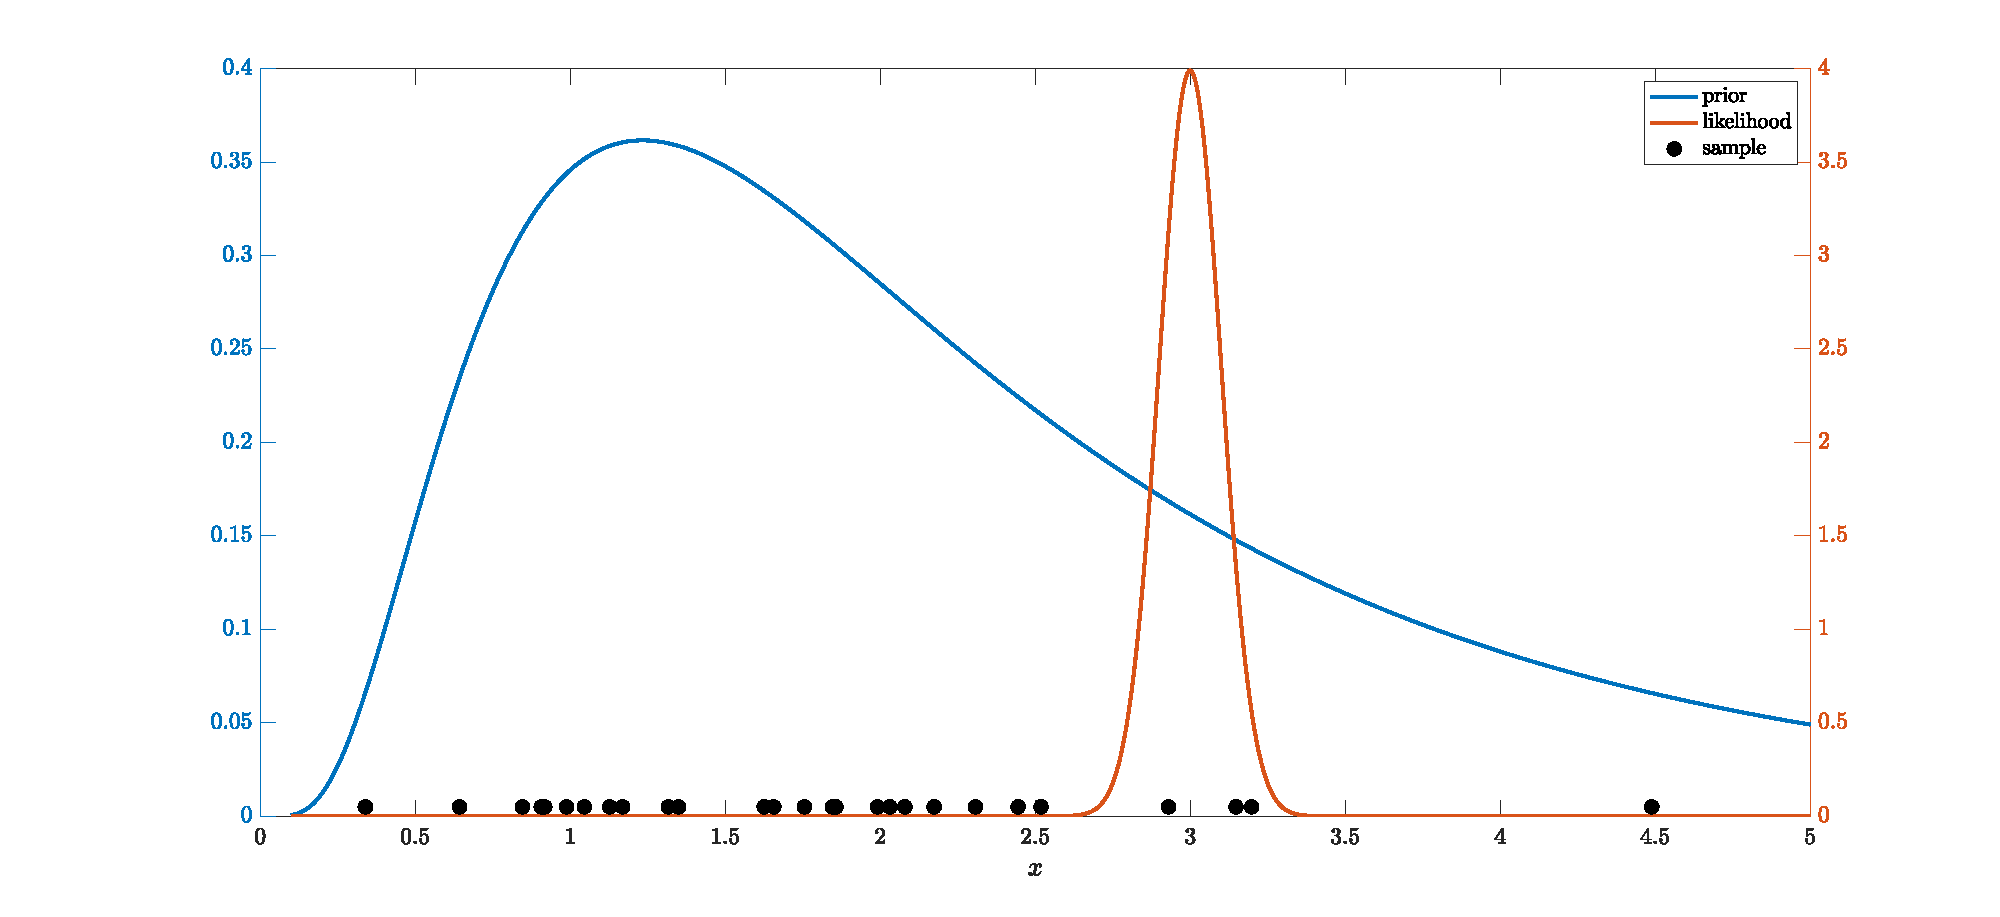
\includegraphics[width = \linewidth]{pf_degen.pdf}
    \caption{Particle degeneracy, shown in a one-dimensional example with 30 particles.}
    \label{fig:pf-degen}
\end{figure}
There are three possible ways to minimalize particle degeneracy: the most obvious one is to have more particles (populate the state space more densely). However, in higher dimensions this demands exponentially more particles. Another solution is to use a different proposal density, therefore having a different likelihood function. In this way the target distribution could be more effectively represented by particles. The third one is resampling: having more particles on top of each other in the same place is better than having only a few of them, while all the others are spread across the domain with negligible weights.


Although particle filters demand low computational power, this only holds when the algorithm is properly tuned, therefore requires the minimal amount of particles. A poor choice of a particle filter, or a poorly designed particle filter requires a lot of computational capacity to give proper results: the particle requirement can be in the order of millions. As were mentioned in \cite{Daum2003}, ``for typical low dimensional tracking problems, the PF requires 2 to 6 orders of magnitude more computer throughput than the extended Kalman filter, to achieve the same accuracy.''

\subsection{The Daum--Huang Filters}
\subsubsection{Main concepts}
To overcome the  undesirable properties of the particle filters (especially the curse of dimensionality), Daum and Huang proposed a new method, where the state estimation is based on log-homotopy based particle flow \cite{Daum2007}. This new filtering method is called Daum-Huang filter (DHF) \cite{Choi2011}.

In particle filters, the problem lies where the Bayes' law is performed to obtain the posterior (this is done though weighting). Upon resampling, the particles ``jump'' from the prior to the posterior. The main concept behind the DHF is to eliminate this often faulty ``jump'', and handle it as a continuous movement. Consider a homotopy in $\lambda$, based on the logarithmic form of the Bayes' law:
\begin{equation}\label{eq:bayes-loghom}
    \log p(\mathbf{x},\lambda) = \log g(\mathbf{x}) + \lambda \log h(\mathbf{x}) - \log K(\lambda),
\end{equation}
where $g(.)$ is the prior, $h(.)$ is the likelihood, $K(.)$ is a normalization constant, and $\lambda$ is the parameter of the homotopy: $\lambda \in [0,1]$. As $\lambda$ changes continuously form 0 to 1, $p(.)$ changes from being the prior $g(.)$, to becoming the posterior, as $\lambda = 1$ (this gives back the standard Bayes' rule). This is essentially the time evolution (in this case $\lambda$ is \emph{pseudotime}) of $p(.)$. Meanwhile the particles that represent the probability distribution also have to move: this movement is described by a stochastic law of motion, with $\lambda$ as the time variable. The question is that how to move these particles according to the also evolving probability distribution, from which they were sampled.

It is assumed that the particles are moving according to the following (It\^{o}) stochastic  differential equation:
\begin{equation}\label{eq:dhf-sde}
    \mathrm{d} \mathbf{x}=\mathbf{f}(\mathbf{x}, \lambda) \mathrm{d} \lambda+\boldsymbol{\sigma}(\mathbf{x}, \lambda) \mathrm{d} \mathbf{W}_{\lambda},
\end{equation}
where $\mathbf{f}(\mathbf{x},\lambda)$ is the drift coefficient,
$\boldsymbol\sigma(\mathbf{x},\lambda)$ is the diffusion coefficient,
and $\mathbf{W}_\lambda$ denotes the standard Brownian motion (Wiener process) in
pseudotime $\lambda$.

The evolution of a probability density under the governing SDE \eqref{eq:dhf-sde} is described by the Fokker--Planck equation, if $\mathbf{x} \in \mathbb{R}^d$:

\begin{equation}\label{eq:fpe}
    \frac{\partial p(\mathbf{x},\lambda)}{\partial \lambda} = -\sum_{i = 1}^{d}\frac{\partial}{\partial x_i}\left[f_i(\mathbf{x},\lambda)p(\mathbf{x},\lambda)\right] + \frac{1}{2}\sum_{i = 1}^{d}\sum_{j = 1}^{d}\frac{\partial^2}{\partial x_i \partial x_j}\left[B_{i,j}(\mathbf{x},\lambda)p(\mathbf{x},\lambda)\right],
\end{equation}
where
\begin{equation}\label{key}
    \mathbf{B} = \frac{1}{2}\boldsymbol\sigma\boldsymbol\sigma^\top.
\end{equation}
Now if \eqref{eq:bayes-loghom} is partially derivated according to $\lambda$, it can be substituted into the left hand side of \eqref{eq:fpe}. After some simplification, the flow equation in its final form:
\begin{align}\label{eq:dhf-eq}
    \log h(\mathbf{x}) - \frac{\partial \log K(\lambda)}{\partial \lambda} & = -\mathbf{f}^\top(\mathbf{x},\lambda)\cdot\nabla\log p(\mathbf{x},\lambda) - \nabla\cdot \mathbf{f}(\mathbf{x},\lambda)       \\
                                                                           & + \frac{1}{2p(\mathbf{x},\lambda)}\left(\nabla^\top\mathbf{B}(\mathbf{x},\lambda)p(\mathbf{x},\lambda)\nabla\right). \nonumber
\end{align}

The main difference between different DHF realizations is the method to solve \eqref{eq:dhf-eq} for $\mathbf{f}(.)$. This is still open question, and holds many room for innovation even to this day.  Here, only the exact flow simplification \cite{Daum2010} is discussed, where the diffusion term ($\boldsymbol\sigma$) is neglected.

\subsubsection{The Exact Flow Daum--Huang Filter}

Under the criteria, that $g(\mathbf{x})$ and $h(\mathbf{x})$ (the prior and the likelihood, essentially the motion model and the measurement model respectively) are Gaussian,
they can be expressed as:
\begin{align}
    \log g(\mathbf{x}) & =-\frac{1}{2}(\mathbf{x}-\phi(\mathbf{x}',\mathbf{u}',0))^{\top} \mathbf{Q}^{-1}(\mathbf{x}-\phi(\mathbf{x}',\mathbf{u}',0)),            \\
    \log h(\mathbf{x}) & =-\frac{1}{2}(\mathbf{z}'-\psi(\mathbf{x},0))^{\top} \mathbf{R}^{-1}(\mathbf{z}'-\psi(\mathbf{x},0)). \label{eq:explicit-log-likelihood}
\end{align}
Then the solution of \eqref{eq:dhf-eq} has the form of
\begin{equation}\label{eq:edh-flow-vector}
    \mathbf{f}(\mathbf{x},\lambda) = \mathbf{C}(\lambda)\mathbf{x} + \mathbf{c}(\lambda),
\end{equation}
where
\begin{align}
     & \mathbf{C}(\lambda) = -\frac{1}{2}\mathbf{\mathbf{\overline\Sigma}}\nabla \psi_x^\top\left(\lambda \nabla \psi_x\mathbf{\overline\Sigma}\nabla \psi_x^\top + \mathbf{R}\right)^{-1}\nabla \psi_x,\label{eq:edh-C}                              \\
     & \mathbf{c}(\lambda) = \left(\mathbf{I}+2\lambda\mathbf{C}\right)\left[\left(\mathbf{I}+\lambda\mathbf{C}\right)\mathbf{\overline\Sigma}\nabla \psi_x^\top\mathbf{R}^{-1}\mathbf{z}' + \mathbf{C}\overline{\mathbf{x}}\right]. \label{eq:edh-c}
\end{align}
Here, $\overline{\mathbf{x}}$ denotes the state average across all the particles for $\lambda = 0$ at a given timestep,
and $\nabla \psi_x$ is the Jacobian of the measurement function, performed around $\overline{\mathbf{x}}_\lambda$,
which is the particle state average for the given $\lambda$.

By solving for $\mathbf{f}(\mathbf{x},\lambda)$,
the state flow vector is obtained according to \eqref{eq:dhf-sde}.
Recall that for the exact flow simplification, the diffusion term $\boldsymbol\sigma$ is
neglected, resulting
\begin{equation}
    \frac{\mathrm{d}\mathbf{x}}{\mathrm{d}\lambda} = \mathbf{f}(\mathbf{x},\lambda).
\end{equation}
Now the motion of the particles is easily described in pseudotime $\lambda$.

The Exact Flow Daum--Huang Filter (EDH) algorithm is summarized as follows.
In one timestep, first the particles are propagated just like in the case of the PF, then $\overline{\mathbf{\Sigma}}$ is calculated using the prediction part of an EKF/UKF.  After this, the homotopy is discretized: $\lambda$ is equally divided into a certain amount of steps. For each \emph{pseudotime} step, $\nabla \psi_x$ is calculated  by linearization around the current state average of the particles, then using the predicted covariance $\overline{\mathbf{\Sigma}}_t$, the measurement $\mathbf{z}'_t$, the measurement noise covariance $\mathbf{R}_t$, and the state average $\overline{\mathbf{x}}_\lambda$, $\mathbf{C}(\lambda)$ and $\mathbf{c}(\lambda)$ is calculated. By this, the drift function $\mathbf{f}(.)$ is obtained. Now, a simple Euler step yields the new state of the particles. Lastly, $\overline{\mathbf{x}}_\lambda$ is re-evaluated. This is repeated for all $\lambda$. It is important to mention that during the homotopy, the time does not change, only the pseudotime $\lambda$. When $\lambda$ has reached 1, the particles are in the position where they estimate the posterior distribution. Now, the state estimation at $t$ can be calculated by taking the average of the particles. Finally, the EKF/UKF update is performed. This was one time step (and along with it, 10 pseudotime step) of the EDH filter.

Figure \ref{fig:dhf-ill}. illustrates the particle flow of the EDH. The time is fixed, and the homotopy is performed from $\lambda = 0$ to $\lambda = 1$. At $\lambda = 1$, the particles moved from the predicted belief (prior, in this context) to their position where they represent the posterior. The true state is indicated by a red square, while the orange dot is the average of the particles. The red arrows show the value of the drift coefficient $\mathbf{f}(\mathbf{x},\lambda)$. As $\lambda$ evolves, the particle average gets closer and closer to the (unknown) true position.

\begin{figure}
    \centering
    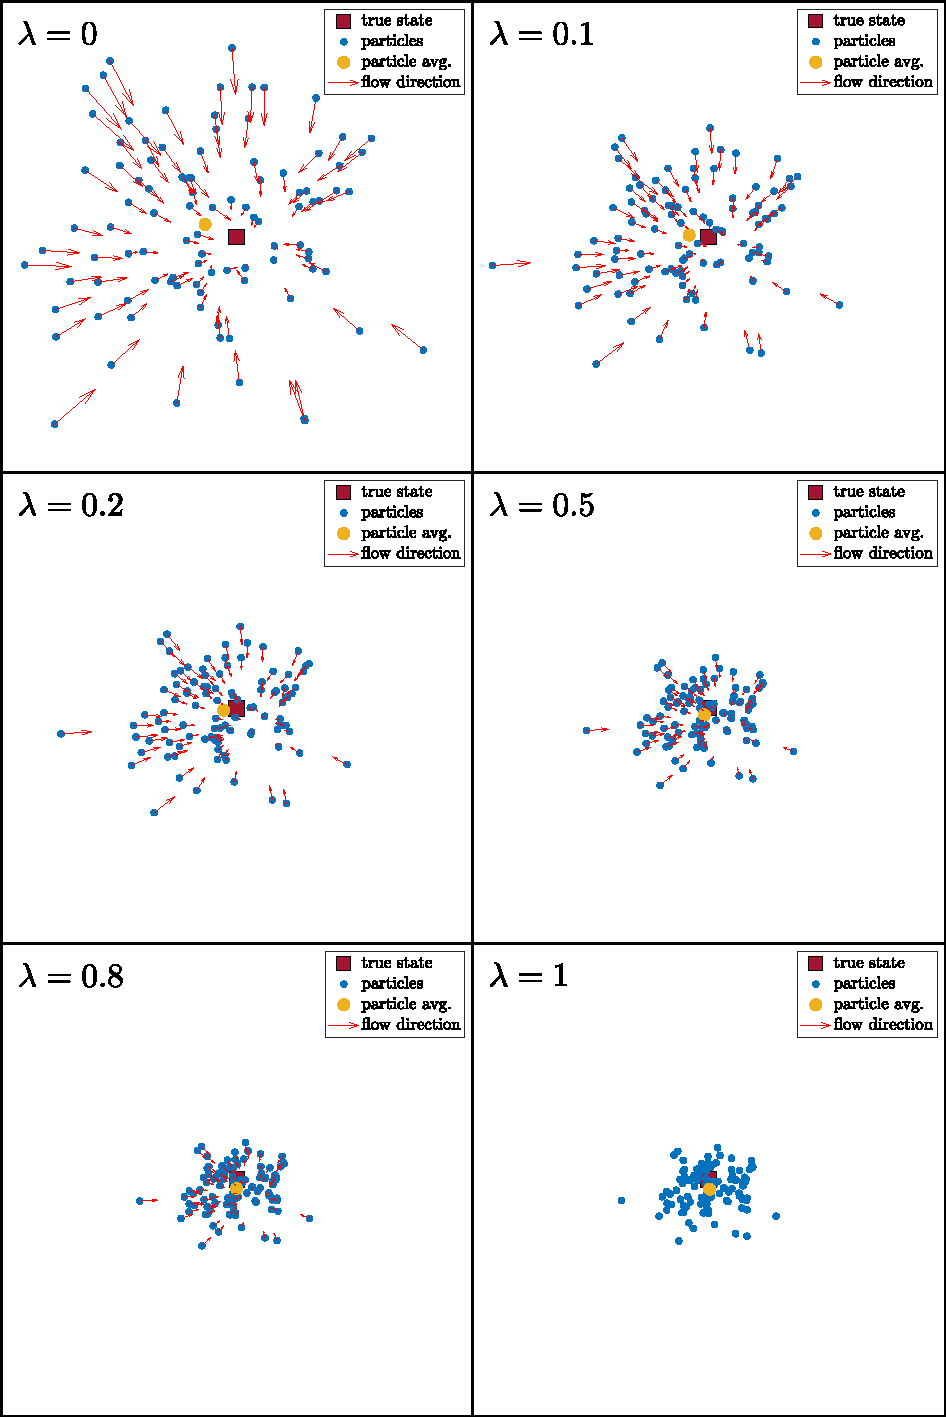
\includegraphics[width=0.98\linewidth]{DHF-visu1.pdf}
    \caption{The particle flow of the EDH. The time is at a fixed value, while the homotopy is performed from $\lambda = 0$ to $\lambda = 1$.}
    \label{fig:dhf-ill}
\end{figure}

\subsubsection{EDH for Implicit Measurement Equation}

Similarly to the case of the EKF, the discussed EDH filter in its original form is not capable of
handling implicit measurement equations.
In \cite{Zhang2012}, the formula for the implicit EKF is derived,
which serves as a foundation for the implicit EDH.

Take the observation function of \eqref{eq:observation-function},
and expand it into a Taylor series about the predicted state, and the measurement at time $t$ $\left(\overline{\boldsymbol\mu}_t,\mathbf{z}'_t\right)$:
\begin{align}
    \psi(\mathbf{x}_t,\mathbf{z}_t) = \psi(\overline{\boldsymbol\mu}_t,\mathbf{z}'_t)
    + \frac{\partial \psi(\overline{\boldsymbol\mu}_t,\mathbf{z}'_t)}{\partial \mathbf{x}_t}(\mathbf{x}_t-\overline{\boldsymbol\mu}_t)
    + \frac{\partial \psi(\overline{\boldsymbol\mu}_t,\mathbf{z}'_t)}{\partial \mathbf{z}_t}(\mathbf{z}_t-\mathbf{z}'_t) \\
    + \mathcal{O}((\mathbf{x}_t-\overline{\boldsymbol\mu}_t)^2)
    + \mathcal{O}((\mathbf{z}_t-\mathbf{z}'_t)^2) \nonumber.
\end{align}

By omitting the higher order terms, rearranging the equation, and also using that \linebreak
$\psi(\mathbf{x}_t,\mathbf{z}_t) = 0$:
\begin{align}
     & \frac{\partial \psi(\overline{\boldsymbol\mu}_t,\mathbf{z}'_t)}{\partial \mathbf{x}_t}\overline{\boldsymbol\mu}_t
    - \psi(\overline{\boldsymbol\mu}_t,\mathbf{z}'_t) = \underbrace{\frac{\partial \psi(\overline{\boldsymbol\mu}_t,\mathbf{z}'_t)}{\partial \mathbf{x}_t}}_{\nabla \psi_x}\mathbf{x}_t + \underbrace{\frac{\partial \psi(\overline{\boldsymbol\mu}_t,\mathbf{z}'_t)}{\partial \mathbf{z}_t}}_{\nabla \psi_z}\underbrace{(\mathbf{z}_t-\mathbf{z}'_t)}_{\mathbf{w}_t}, \\
     & \mathbf{y}_t :=  \frac{\partial \psi(\overline{\boldsymbol\mu}_t,\mathbf{z}'_t)}{\partial \mathbf{x}_t}\overline{\boldsymbol\mu}_t
    - \psi(\overline{\boldsymbol\mu}_t,\mathbf{z}'_t) = \nabla\psi_x(\overline{\boldsymbol\mu}_t,\mathbf{z}'_t)\overline{\boldsymbol\mu}_t-\psi(\overline{\boldsymbol\mu}_t,\mathbf{z}'_t) \label{eq:edh-implicit-y}.
\end{align}
As a result, a linear measurement equation is obtained, similarly to \eqref{eq:lin-meas-model}:
\begin{equation}
    \mathbf{y}_t = \nabla \psi_x \mathbf{x}_t + \nabla \psi_z\mathbf{w}_t,\quad\quad \mathbf{w}_t \sim \mathcal{N}(0,\mathbf{R}).
\end{equation}

For this formulated explicit measurement equation, \eqref{eq:explicit-log-likelihood} can be written as
\begin{equation}
    \log h(\mathbf{x}) =-\frac{1}{2}(\mathbf{y}-\nabla \psi_x \mathbf{x}_t)^{\top} (\nabla \psi_z\mathbf{R}\nabla \psi_z^{\top})^{-1}(\mathbf{y}-\nabla \psi_x \mathbf{x}_t).
\end{equation}

Now carrying on with the derivation in \cite{Khan2018} with this modified log-likelihood,
the altered form of \eqref{eq:edh-C} and \eqref{eq:edh-c} for an implicit measurement
equation is:
\begin{align}
     & \mathbf{C}(\lambda) = -\frac{1}{2}\mathbf{\mathbf{\overline\Sigma}}\nabla \psi_x^\top\left(\lambda \nabla \psi_x\mathbf{\overline\Sigma}\nabla \psi_x^\top + \nabla \psi_z\mathbf{R}\nabla \psi_z^{\top}\right)^{-1}\nabla \psi_x,  \label{eq:edh-C-impl}                             \\
     & \mathbf{c}(\lambda) = \left(\mathbf{I}+2\lambda\mathbf{C}\right)\left[\left(\mathbf{I}+\lambda\mathbf{C}\right)\mathbf{\overline\Sigma}\nabla \psi_x^\top(\nabla \psi_z\mathbf{R}\nabla \psi_z^{\top})^{-1}\mathbf{y} + \mathbf{C}\overline{\mathbf{x}}\right]. \label{eq:edh-c-impl}
\end{align}
\subsubsection{Other Daum--Huang Filter Variants}

Solving \eqref{eq:dhf-eq} requires various simplifications. Assuming exact flow, where the diffusion part is neglected (only deterministic flow is considered), the measurement model is linear (or linearized), and the noise acting on the system is a Gaussian random variable (or from the exponential family) is only one variation of the Daum--Huang filter. When the linearization of the measurement function is performed around the location of \emph{each} particle instead of their average, the local exact flow Daum--Huang filter is constructed \cite{Ding2012}. Particle weighting can be developed for Daum--Huang filters as well, proposed in \cite{Li2016}.

Another simplification is the assumption of incompressible flow \cite{Daum2007}  (this was the first type of the Daum--Huang filter), the assumption of geodesic flow \cite{Daum2013}, and the latest results are from the consideration of stochastic particle flow (the diffusion term is no longer neglected), using Gromov's method \cite{Daum2018,Dai2021}.

It is difficult to summarize the performance of Daum--Huang filters, so is the case with particle filters. Many realizations exist, each with they own advantages and disadvantages. The main problem is with computational capacity: a method with much more advanced and/or more precise calculations can yield better results at a cost of computational time. The main challenge is to develop algorithms and variations that does not require significantly more computation, yet result in a more robust and more precise estimation of the state.

\subsection{Realization of the EDH for the Inspected Localization Problem}

The original EDH algorithm for implicit measurement equation is described
in \cite{Ding2012}.
Now, that the implicit EDH is introduced along with the motion and measurement models
for the localization problem in scope, the full algorithm for the EDH can be formulated.
Algorithm \ref{alg:edh-loc}. contains one step of the filter.
For each computation, the relevant equations are indicated at the end of the line.
The resulting estimated state is $\overline{\mathbf{x}}_t$, which is then used to evaluate the performance of the proposed method in the next section.
\begin{algorithm}
    \caption{Exact Flow Daum--Huang Filter for Localization($\boldsymbol{\mu}_{t-1},\mathbf{\Sigma}_{t-1},\hat{\mathbf{u}}_t,\mathbf{z}'_t,\{\mathbf{x}_t^i\}_{i=1}^{N}$)}\label{alg:edh-loc}
    \begin{algorithmic}[1]
        \If{t is 0} \Comment{initialization step}
        \State Draw $N$ particles from a prior distribution: $\{\mathbf{x}_0^i\}_{i=1}^{N}$;
        \State Calc. the mean $\boldsymbol\mu_0$ and covar. $\boldsymbol\Sigma_0$ of the particle set, assign $\overline{\mathbf{x}}_0 = \boldsymbol{\mathbf{\mu}}_0$;
        \State\Return $\boldsymbol{\mu}_0,\boldsymbol{\Sigma}_0,\{\mathbf{x}_0^i\}_{i=1}^{N},\overline{\mathbf{x}}_0$;
        \EndIf
        \State Calculate $\mathbf{u}_t$, using $\hat{\mathbf{u}}_t$; \Comment{\eqref{eq:odom-raw-input}-\eqref{eq:odom-delta-input}}
        \State Calculate $\mathbf{Q}_t$ using $\mathbf{u}_t$
        \Comment{\eqref{eq:control-covar}}
        \State Propagate particles: $\mathbf{x}_t^{i} = \phi(\mathbf{x}_{t-1}^{i},\mathbf{u}_t,\mathbf{v}_t)$;
        \Comment{\eqref{eq:prop-x}-\eqref{eq:prop-theta}}
        \State Calculate the average of the particle set $\{\mathbf{x}_t^i\}_{i=1}^{N}$: $\overline{\mathbf{x}}_t$;
        \State Assign $\overline{{\mathbf{x}}}_{t,0} = \overline{\mathbf{x}}_t$;
        \State EKF prediction:
        \State\indent Evaluate the Jacobians at $(\boldsymbol{\mu}_{t-1},\mathbf{u}_t)$:
        \Comment{\eqref{eq:motmodel-jacobi-x}-\eqref{eq:motmodel-jacobi-u}}
        \State\indent\indent $\nabla\phi_x := \nabla\phi_x(\boldsymbol{\mu}_{t-1},\mathbf{u}_t),\quad \nabla\phi_u := \nabla\phi_x(\boldsymbol{\mu}_{t-1},\mathbf{u}_t)$;
        \State\indent$\overline{\boldsymbol{\mu}}_t = \phi(\boldsymbol{\mu}_{t-1},\mathbf{u}_t,\mathbf{v}_t = 0)$;
        \State\indent
        $\overline{\mathbf{\Sigma}}_t = \nabla \phi_x\mathbf{\Sigma}_{t-1}\nabla \phi_x^{\top}
            +\nabla \phi _u\mathbf{Q}_t \nabla \phi_u^{\top}$;
        \For{$j = 1\dots N_{\lambda}$} \Comment{$N_{\lambda}:$ number of $\lambda$ steps}
        \State $\lambda = j\Delta\lambda$;
        \Comment{$\Delta\lambda$: step size}
        \State Evaluate $\nabla\psi_x(\overline{\mathbf{x}}_t,\mathbf{z}'_t),\nabla\psi_z(\overline{\mathbf{x}}_t,\mathbf{z}'_t)$;
        \Comment{\eqref{eq:measmodel-jacobi-x}-\eqref{eq:measmodel-jacobi-z}}
        \State Calculate $\mathbf{y}_t$, using $\overline{\mathbf{x}}_t,\mathbf{z}'_t$,$\nabla\psi(\overline{\mathbf{x}}_t,\mathbf{z}'_t)$; \Comment{\eqref{eq:edh-implicit-y},\eqref{eq:observation-function}}
        \State Calculate $\mathbf{C}$ and $\mathbf{c}$, using
        $\lambda,\overline{\boldsymbol\Sigma}_t, \overline{\mathbf{x}}_{t,0}$,
        $\nabla\psi_x(\overline{\mathbf{x}}_t,\mathbf{z}'_t),\nabla\psi_z(\overline{\mathbf{x}}_t,\mathbf{z}'_t), \mathbf{y}_t$;
        \Comment{\eqref{eq:edh-C-impl}-\eqref{eq:edh-c-impl}}
        \State Evaluate $\mathbf{f}(\mathbf{x},\lambda)$ for every particle $\mathbf{x}_t^{i}$, resulting $\frac{\mathrm{d}\mathbf{x}_t^i}{\mathrm{d}\lambda}$;
        \Comment{\eqref{eq:edh-flow-vector}}
        \State Update the pose of each particle by an Euler-step:
        \State\indent $\mathbf{x}_t^{i} = \mathbf{x}_t^{i} + \Delta\lambda\frac{\mathrm{d}\mathbf{x}_t^i}{\mathrm{d}\lambda}$;
        \State Re-evaluate $\overline{\mathbf{x}}_t$ with the updated particle poses;
        \EndFor
        \State EKF update:
        \State\indent Evaluate the Jacobians at $(\overline{\boldsymbol{\mu}}_t,\mathbf{z}'_t)$:
        \Comment{\eqref{eq:motmodel-jacobi-x}-\eqref{eq:motmodel-jacobi-u}}
        \State\indent\indent $\nabla\psi_x := \nabla\psi_x(\overline{\boldsymbol{\mu}}_t,\mathbf{z}'_t), \quad \nabla\psi_u := \nabla\psi_x(\overline{\boldsymbol{\mu}}_t,\mathbf{z}'_t)$;
        \State\indent $\mathbf{K}_t = \overline{\mathbf{\Sigma}}_t\nabla \psi_x^\top\left(\nabla \psi_x\overline{\mathbf{\Sigma}}_t\nabla \psi_z^\top+
            \nabla \psi_z\mathbf{R}\nabla \psi^{\top}_z\right)^{-1}$;
        \State\indent $\boldsymbol{\mu}_t = \overline{\boldsymbol{\mu}}_t + \mathbf{K}_t\left(0-\psi(\overline{\boldsymbol{\mu}}_t,\mathbf{z}'_t)\right)$;
        \Comment{\eqref{eq:observation-function}}
        \State\indent $\mathbf{\Sigma}_t = \left(\mathbf{I}-\mathbf{K}_t\nabla \psi_x\right)\overline{\mathbf{\Sigma}}_t$;
        \State\Return $\boldsymbol{\mu}_t,\boldsymbol{\Sigma}_t,\{\mathbf{x}_t^i\}_{i=1}^{N},\overline{\mathbf{x}}_t$;
    \end{algorithmic}
\end{algorithm}
